\chapter{Introduction}
\label{sec:intro}

Planning under uncertainty is vital in order for a planning algorithm to move
out of the lab and into the real world, as the ideal model for a dynamical
system does not directly translate into successful execution outside of
simulations. There are modeled- and unmodeled uncertainties, sensory noise and
unforseeen environment obstacles and incidents happening all the time that a
planner has to take into account if it whishes to make this jump. Over the last
couple of decades a lot of research has gone in to handling uncertianty in
planning, an overview of which can be found in \cref{chp:survey-of-papers}.

In general planning is harder for a nonlinear and non-holonomic vehicle, such as
the unicycle model employed in this thesis, and imagined to be an airplane.
Especially when uncertainty is added to the model. In this case a lot of
planners simply choose to ignore these error sources and apply heuristics such
as maximizing the distance to the obstacles in the environment. Note that this
is the approach taken by the benchmark planner in the experiments section.
However, this adds the disadvantage that the plans can become overly
conservative. Explicitly handling the uncertanties in the planning stage enables
to planner to employ more aggressive maneuvers, such as flying through two trees
close together, as opposed to flying around the entire grove. Flying straight
through is an acceptable maneuver as the planner has guarantees on the
whereabouts of the dynamical system, and hence is not afraid to go close to an
obstacle. This confidence in planning is enabled by the calculation of
\textit{robust motion primitives} through a \ac{SOS} framework.

\begin{figure}
  \begin{subfigure}{0.5\textwidth}
    \includegraphics[width=\textwidth]{figures/experiments/experiment-setup-no-funnel}
    \caption{The airplane is deviating from the nominal trajectory due to the
      cross-wind.}
  \end{subfigure}%
  \;
  \begin{subfigure}{0.5\textwidth}
    \includegraphics[width=\textwidth]{figures/experiments/experiment-setup-funnel}
    \caption{The reachable set given the cross-wind pictured.}
  \end{subfigure}
  \caption{Not taking uncertainty into account can lead to collisions when the
    actual trajectory diverges from the nominal one.}
\end{figure}

With the advent of \ac{SOS} programming one is now able to search, numerically,
for a Lyapunov function to verify the convergence of the nonlinear feedback
system. The one-level subset of the Lyapunov function is then used as the
reachable set of the dynamical system. Adding uncertainty to the verification is
simply the addition of adding a couple of extra constraints to the \ac{SOS}
program definition.

The \ac{RRT} algorithm can handle large state spaces, and differential
constraints. However, it is not able to directly reason about uncertainty and
feedback during the planning stage. It is therefore that this thesis seeks to
combine the \ac{SOS} programming framework to generate robust motion primitives
for the \ac{RRT} algorithm which will use these primitives during the planning
stage, and hence can act like a normal \ac{RRT} algorithm, yet handle all the
difficulties of uncertainty and feedback at the same time, as this is all
contained in the motion primtives employed as branches in the planning tree.
This combination is dubbed the \rrtfunnel{} algorithm, and is the result of this
thesis, and will be put to test against a benchmark \ac{RRT} algorithm in the
experiment section.


The experiments will be conducted through simulations in a random forest, so
that the airplane model and the planner will have to find its way safely through
a strip of forest if it is to make to the target. A cartoon of the experiment
setup can be found in \cref{fig:experiment-cartoon}.

\begin{figure}
  \centering
  \missingfigure{experiment cartoon}
  \caption{The strip of forest that the airplane has to traverse safely in order
  for the planner to show that it handles uncertainty.}
\label{fig:experiment-cartoon}
\end{figure} 



\section{Outline}

The planning algorithm in this thesis is based on two 

This dissertation draws heavily on the earlier work and writing in the follow-
ing papers, written jointly with several collaborators:

\cite{majumdarFunnelLibrariesRealtime2017}

The rest of the thesis is organised as follows:
\begin{description}
    \item[\cref{chp:survey-of-papers}]
      provides a survey of current motion planning research focused on handling
      uncertainty in the environment, the system state and the surrounding
      environment, as well as some more in depth on the funnel theory employed
      in this thesis.
    
    \item[\cref{chp:preliminaries}]
      provides some introductory theory, first to motion planning as a general
      topic, then introduces the funnel generation theory through \ac{SOS}
      programming, and then develops the basic theory needed for understanding
      the inner workings of the \ac{RRT} algorithm.
    
    \item[\cref{chp:method}]
      develops the \rrtfunnel{} algorithm through two parts. Firstly it develops
      robust motion primtives through the \ac{SOS} programming framework. Then
      it develops the needed heuristics and sampling distribution for the
      \ac{RRT} motion planner and then incorporates the funnels from the first
      part as the extension operators to the tree that the algorithm builds
      through the configuration space.
    
    \item[\cref{chp:experiments}]
      contains the description of how to create and setup the experiment
      environment and the benchmark planner that is used in comparing the
      performance of the \rrtfunnel{} algorithm. The results follow right after.
    
    \item[\cref{chp:discussion}]
      gives a discussion of the results and a pointer to further work on the problem.

    \item[\cref{sec:first-app}]
      gives a basic introduction to the theory of \ac{SOS} verification of
      dynamical systems.

    \item[\cref{AppendixB}]
      contains some code examples from code. The rest of which can be found in \cite{my-code}.

   
\end{description}



